\documentclass[12pt]{article}
\usepackage{graphicx,amsthm,amsmath,amssymb,algorithm,algorithmic,geometry,setspace,fancyhdr,varwidth,subfig,pdfpages,float,verbatim}
\usepackage[english]{babel}
\usepackage[colorlinks=true,linkcolor=blue]{hyperref}
\usepackage[superscript,biblabel]{cite}
\usepackage[export]{adjustbox}
\geometry{letterpaper,
	total={170mm,257mm},
	left=20mm,
	top=30mm, bottom=20mm}  % or letter or a5paper or ... etc
% \geometry{landscape} % rotated page geometry

\title{Ph 20: Assignment \#4}
\author{Maya Fuller}
\date{Due: May 14, 2018} % delete this line to display the current date

% See the ``Article customise'' template for come common customisation

\begin{document}
	
	\pagenumbering{gobble}
	
	\maketitle

	\noindent\textbf{\large Makefile}\\
	\verbatiminput{Makefile}\\
	
	\noindent\textbf{\large Version Control}\\
	\verbatiminput{vc.log}\\
	
	\noindent\textbf{\large Source Code}\\
	\verbatiminput{ode.py}
	
	\noindent\textbf{\large Part 1}\\
	
	\indent\textbf{Problem 1 and 2}\\
		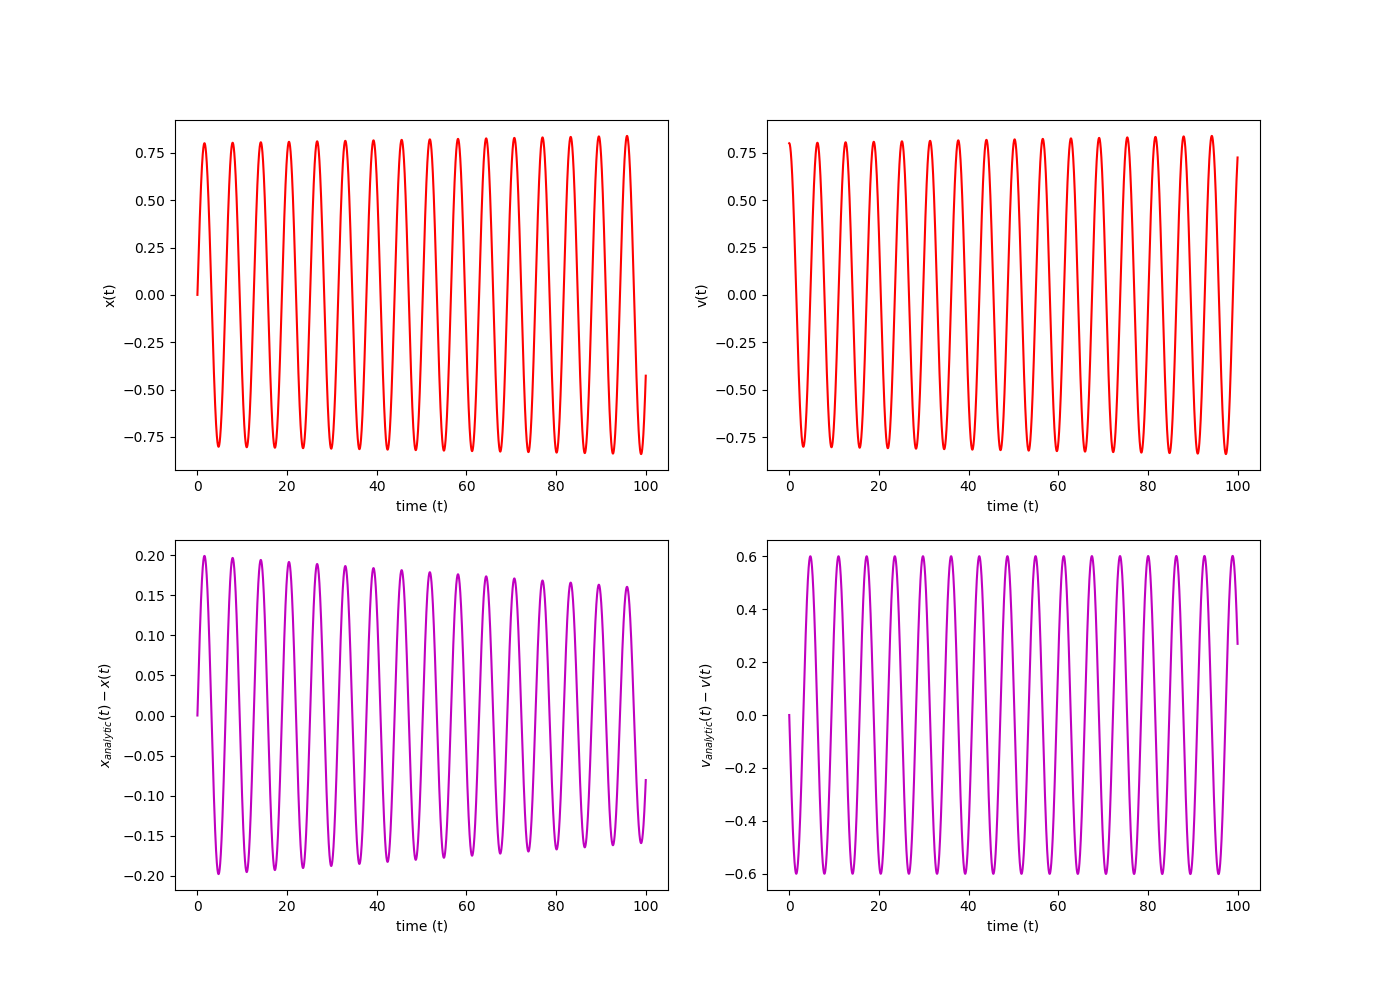
\includegraphics[width=0.9\textwidth]{vstimePlots.png}\\
		
	\indent\textbf{Problem 3}\\
		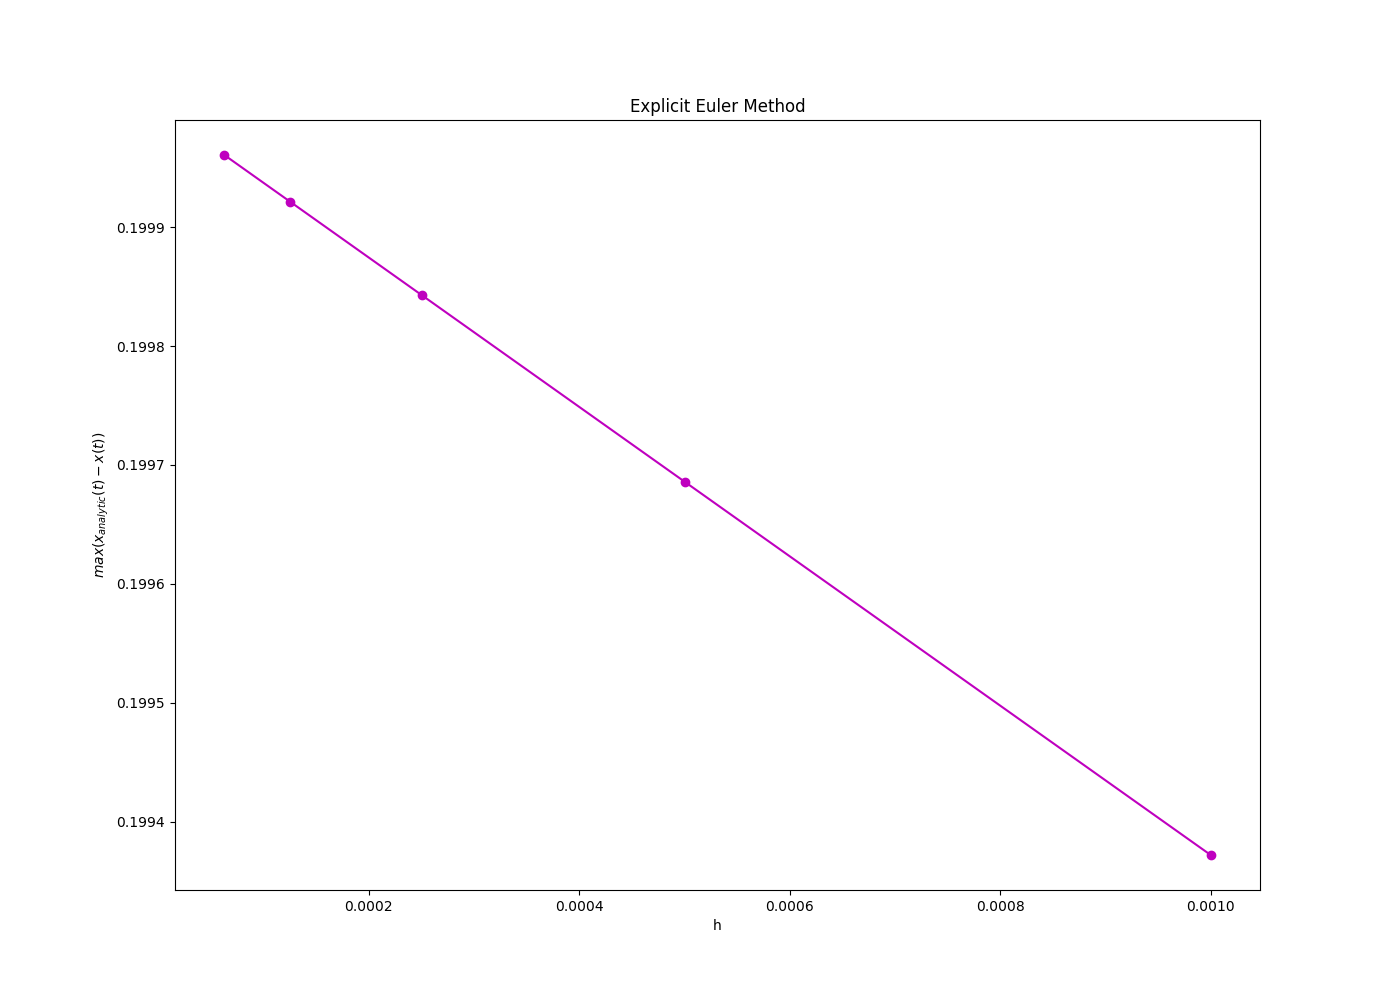
\includegraphics[width=0.9\textwidth]{errorPlot.png}\\
		
	\indent\textbf{Problem 4}\\
		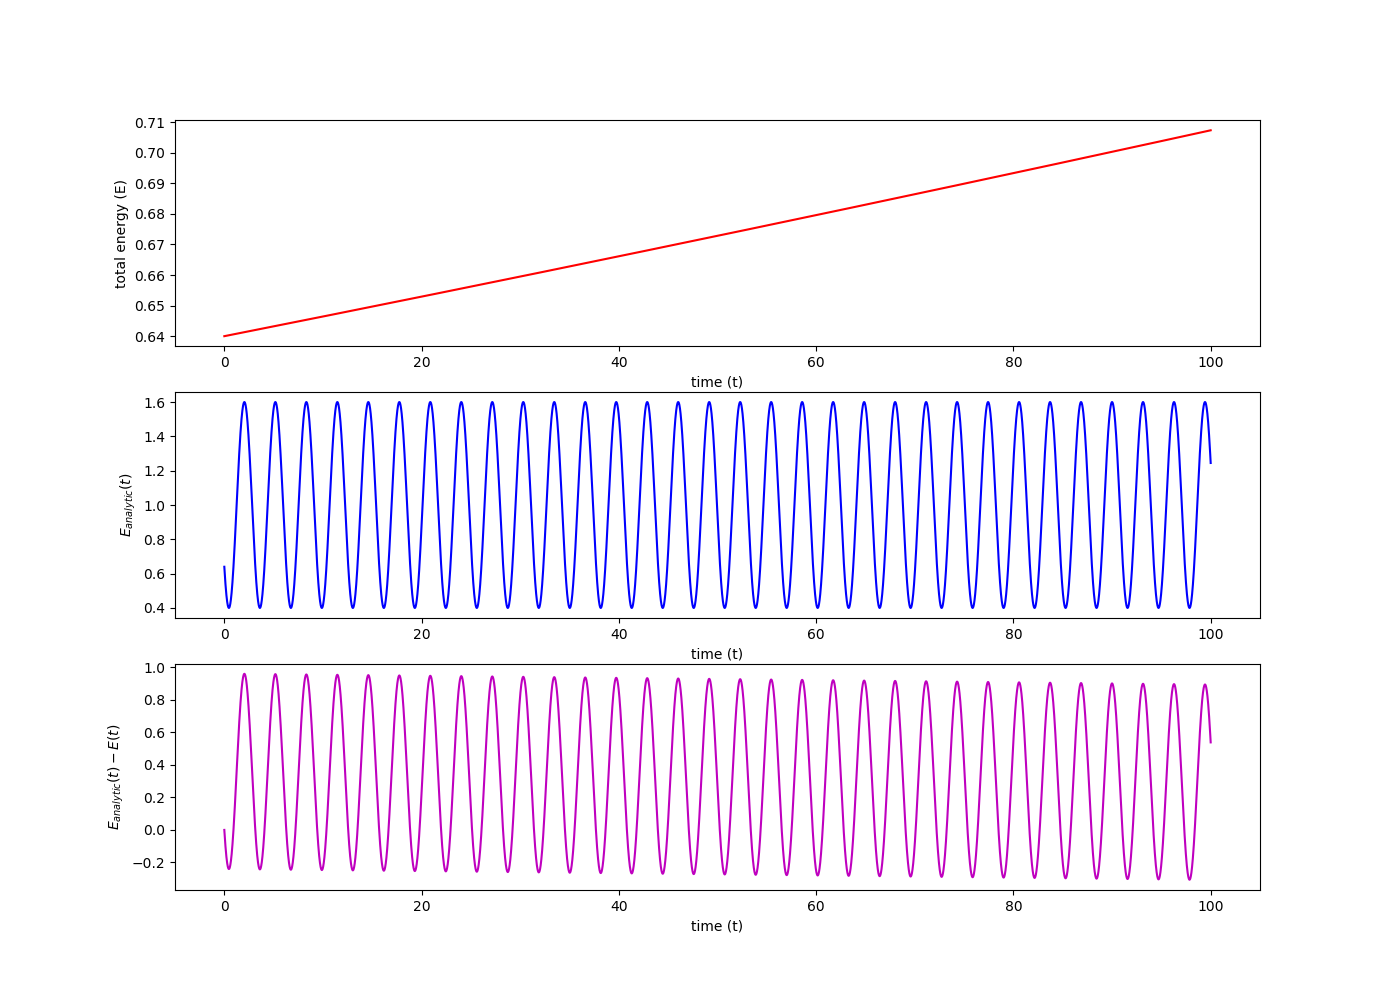
\includegraphics[width=0.9\textwidth]{energyPlot.png}\\
		
	\indent\textbf{Problem 5}\\
		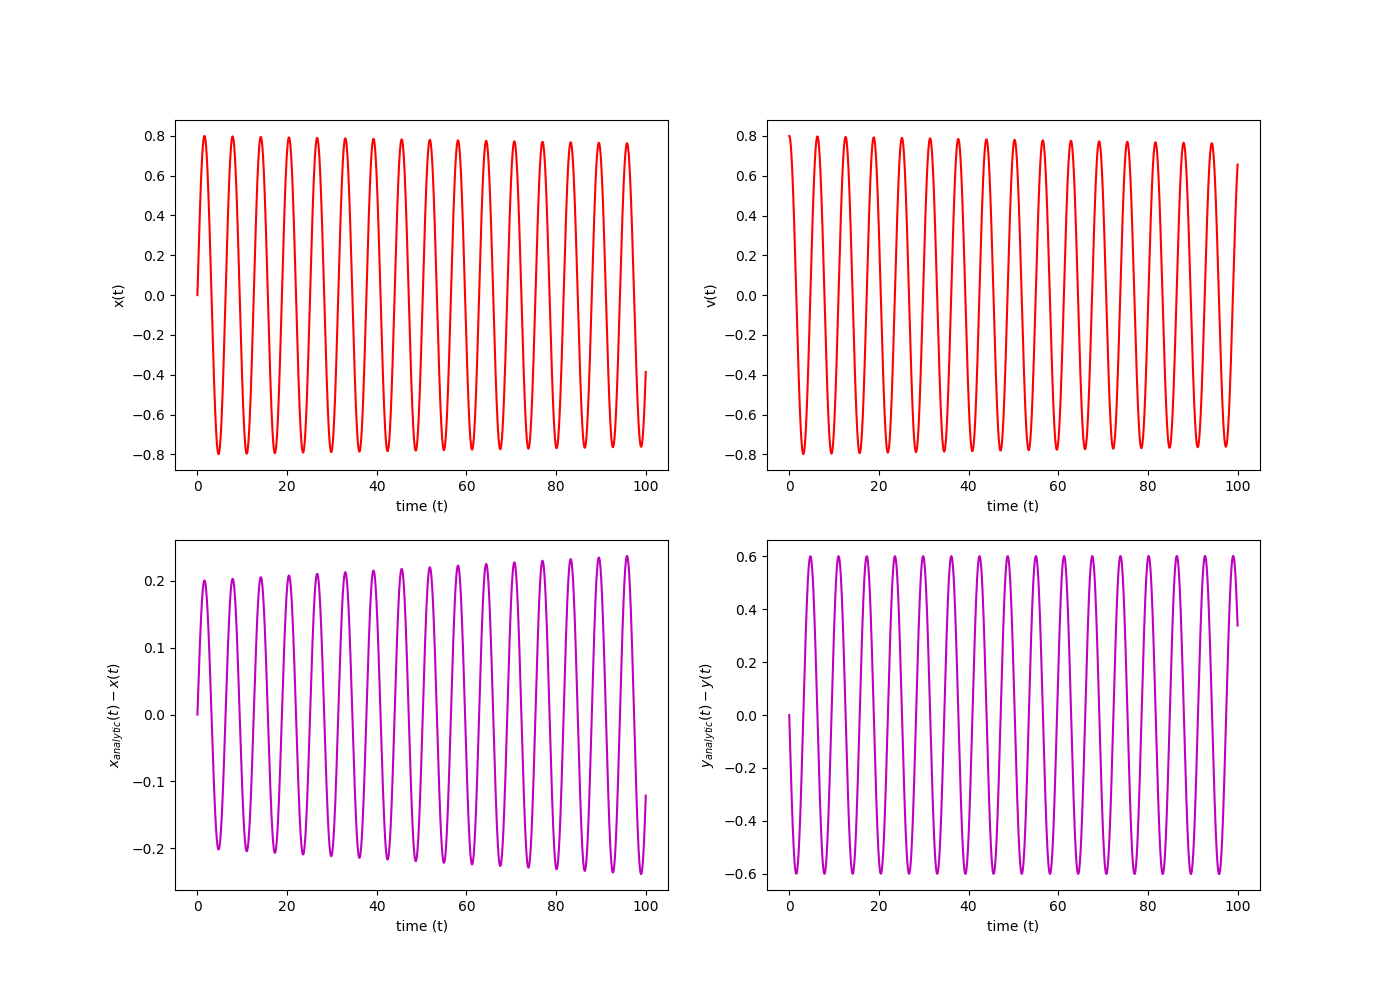
\includegraphics[width=0.9\textwidth]{implicitPlot.png}\\
		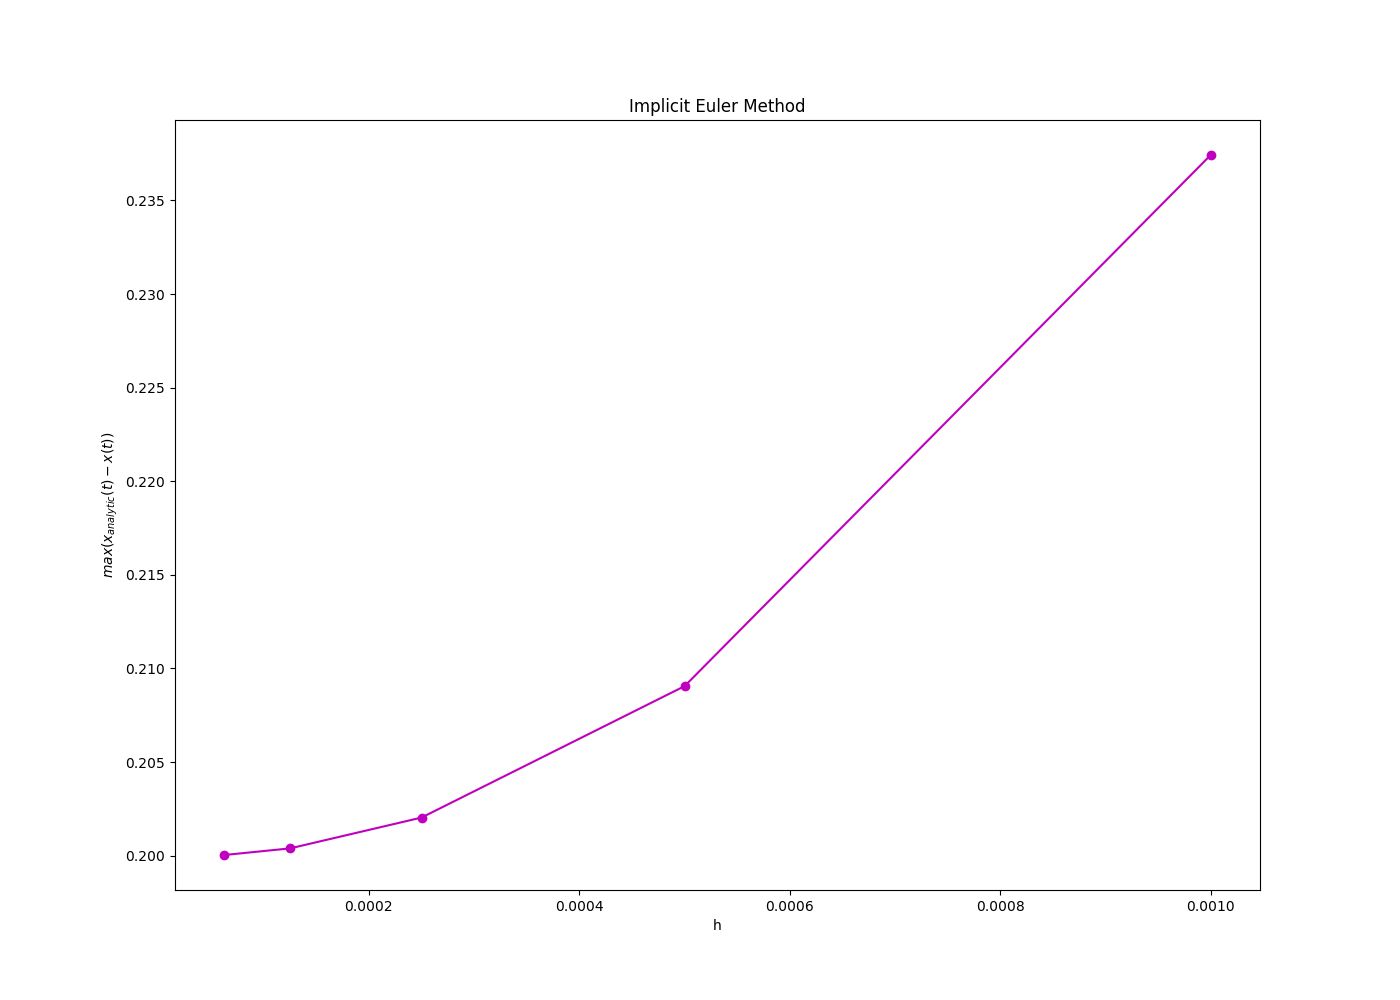
\includegraphics[width=0.9\textwidth]{errorImplicitPlot.png}\\
		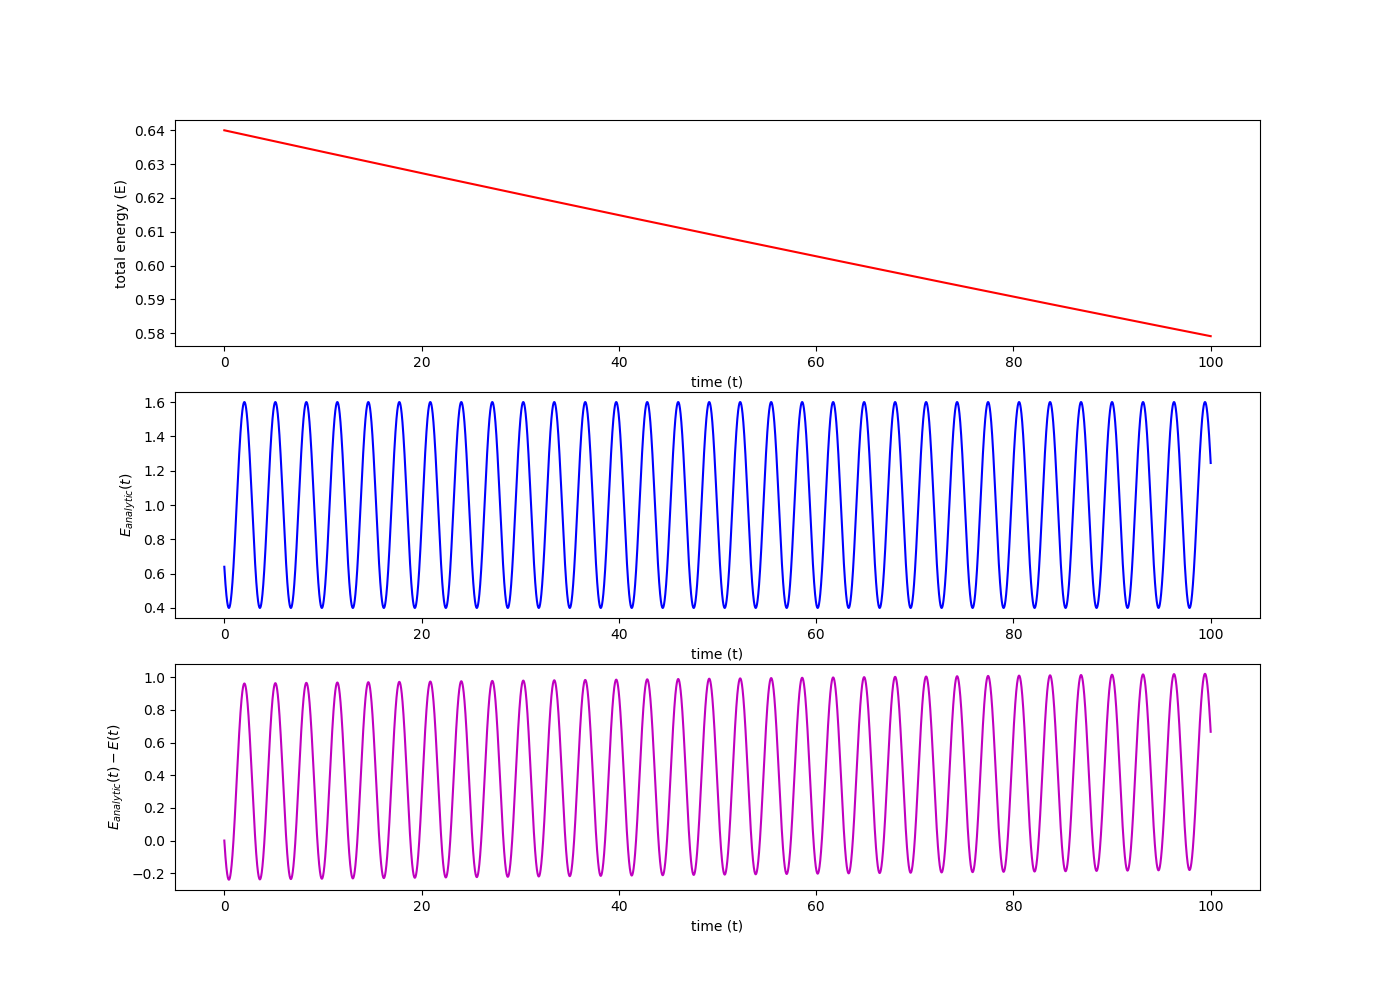
\includegraphics[width=0.9\textwidth]{energyImplicitPlot.png}\\

	\noindent\textbf{\large Part 2}\\
	
	\indent\textbf{Problem 1 and 2}\\
			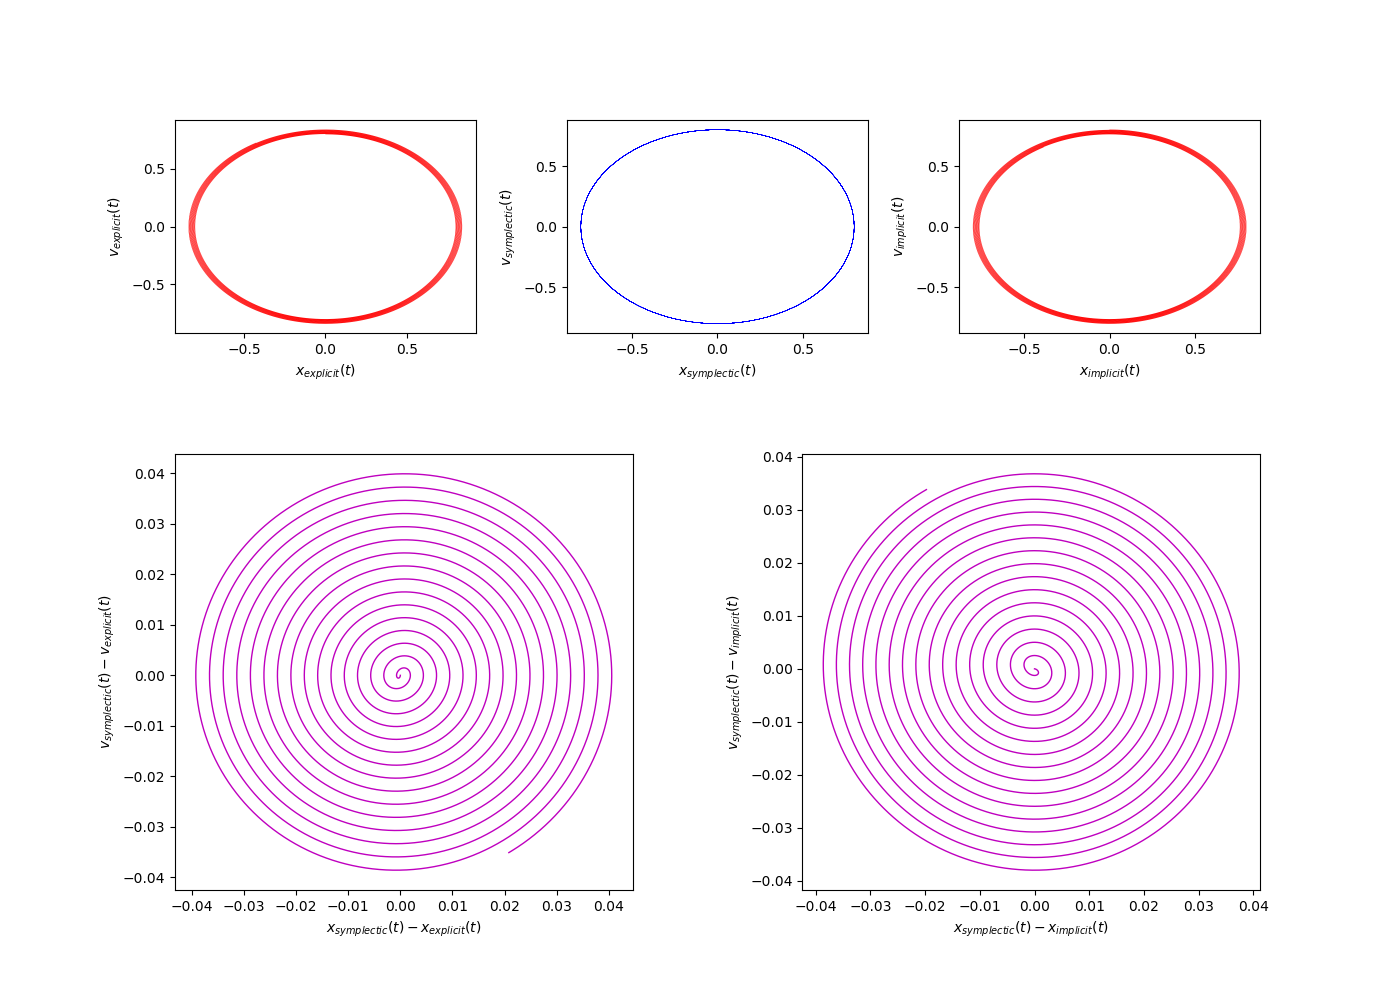
\includegraphics[width=0.9\textwidth]{phaseSpace.png}\\

	\indent\textbf{Problem 3}\\
		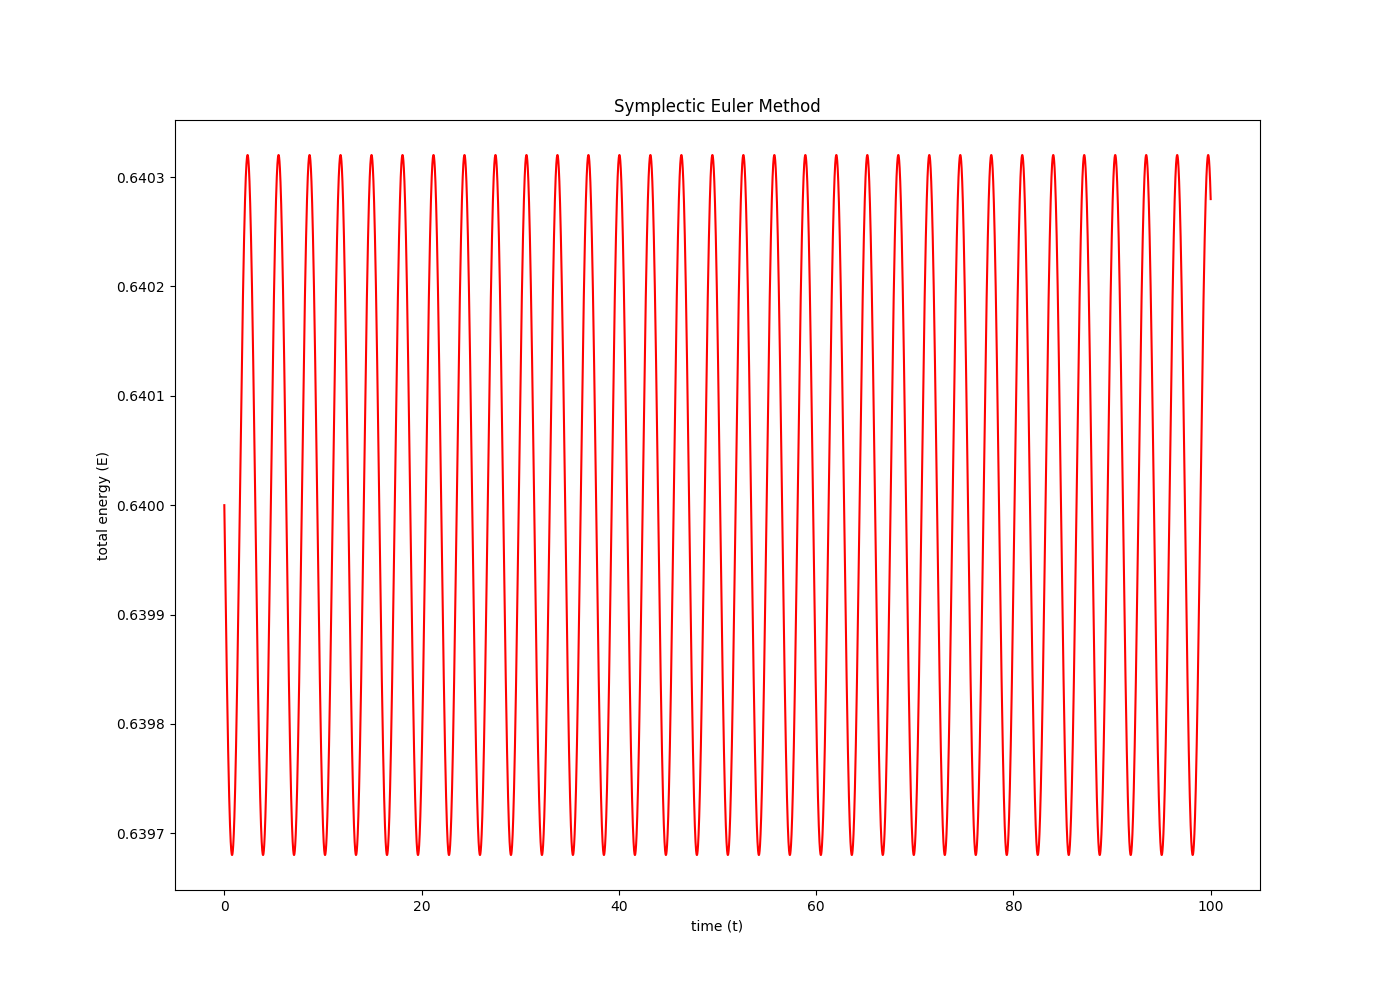
\includegraphics[width=0.9\textwidth]{energySymplecticPlot.png}\\
	
	\indent\textbf{Problem 4}\\
		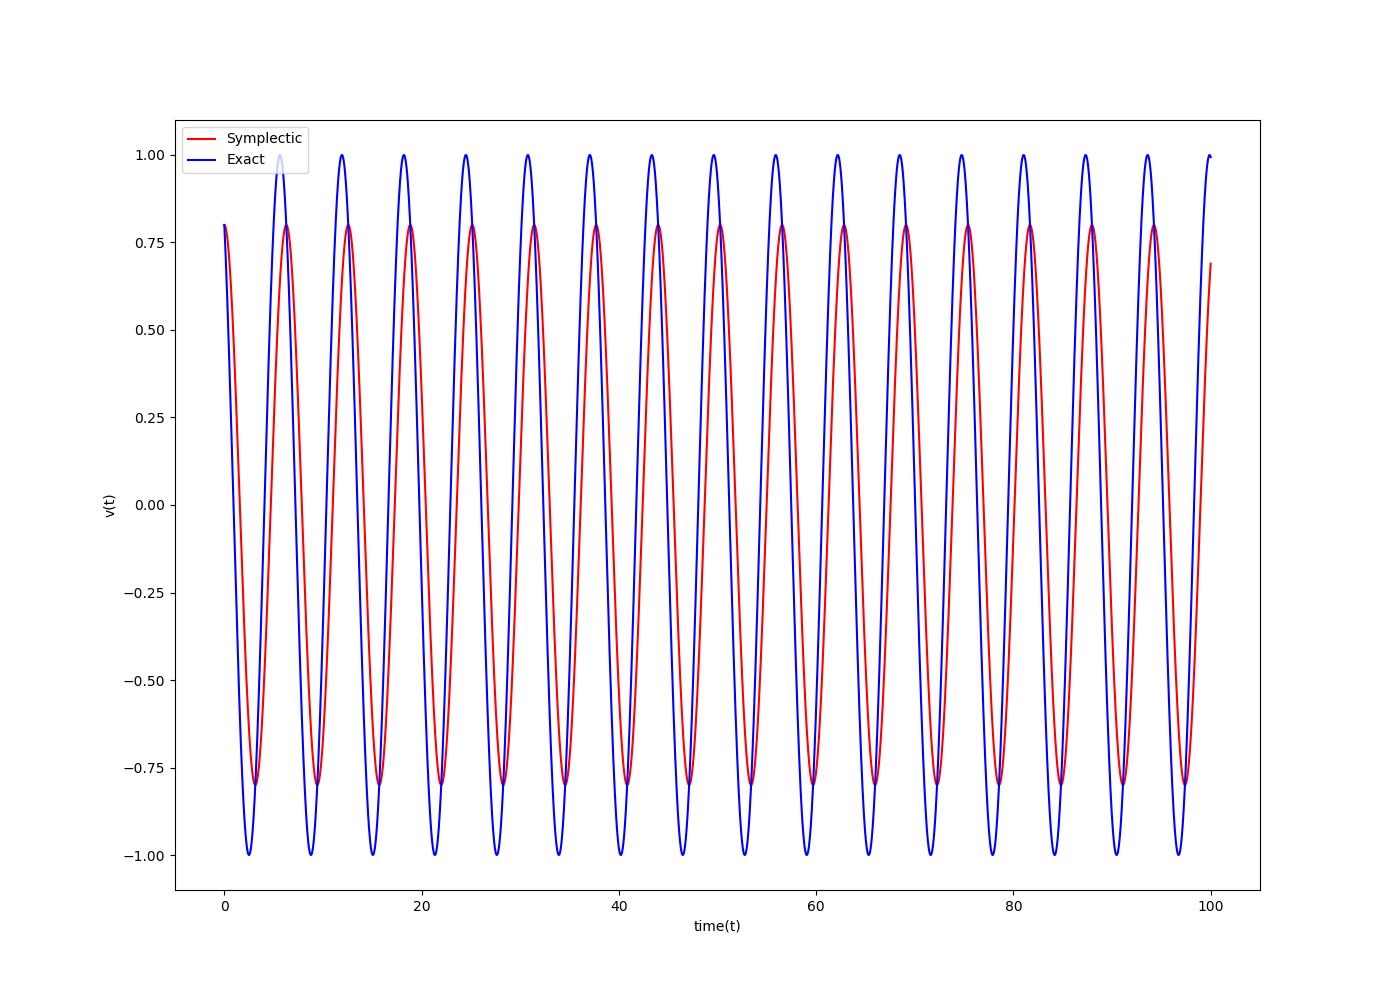
\includegraphics[width=0.9\textwidth]{vSymPlot.png}\\
		
\end{document}